% -*- mode: latex; -*- mustache tags:  
\documentclass[10pt,twoside,english]{_support/latex/sbabook/sbabook}
\let\wholebook=\relax

\usepackage{import}
\subimport{_support/latex/}{common.tex}

%=================================================================
% Debug packages for page layout and overfull lines
% Remove the showtrims document option before printing
\ifshowtrims
  \usepackage{showframe}
  \usepackage[color=magenta,width=5mm]{_support/latex/overcolored}
\fi


% =================================================================
\title{Learning Object-Oriented Programming, Design and TDD with Pharo}
\author{Stéphane Ducasse}
\series{The Pharo TextBook Collection}

\hypersetup{
  pdftitle = {Learning Object-Oriented Programming, Design and TDD with Pharo},
  pdfauthor = {Stéphane Ducasse},
  pdfkeywords = {Introduction, programming, design, testing, Pharo, Smalltalk}
}


% =================================================================
\begin{document}

% Title page and colophon on verso
\maketitle
\pagestyle{titlingpage}
\thispagestyle{titlingpage} % \pagestyle does not work on the first one…

\cleartoverso
{\small

  Copyright 2017 by Stéphane Ducasse.

  The contents of this book are protected under the Creative Commons
  Attribution-ShareAlike 3.0 Unported license.

  You are \textbf{free}:
  \begin{itemize}
  \item to \textbf{Share}: to copy, distribute and transmit the work,
  \item to \textbf{Remix}: to adapt the work,
  \end{itemize}

  Under the following conditions:
  \begin{description}
  \item[Attribution.] You must attribute the work in the manner specified by the
    author or licensor (but not in any way that suggests that they endorse you
    or your use of the work).
  \item[Share Alike.] If you alter, transform, or build upon this work, you may
    distribute the resulting work only under the same, similar or a compatible
    license.
  \end{description}

  For any reuse or distribution, you must make clear to others the
  license terms of this work. The best way to do this is with a link to
  this web page: \\
  \url{http://creativecommons.org/licenses/by-sa/3.0/}

  Any of the above conditions can be waived if you get permission from
  the copyright holder. Nothing in this license impairs or restricts the
  author's moral rights.

  \begin{center}
    
\includegraphics[width=0.2\textwidth]{_support/latex/sbabook/CreativeCommons-BY-SA.pdf}
  \end{center}

  Your fair dealing and other rights are in no way affected by the
  above. This is a human-readable summary of the Legal Code (the full
  license): \\
  \url{http://creativecommons.org/licenses/by-sa/3.0/legalcode}

  \vfill

  % Publication info would go here (publisher, ISBN, cover design…)
  Layout and typography based on the \textcode{sbabook} \LaTeX{} class by Damien
  Pollet.
}


\frontmatter
\pagestyle{plain}

\tableofcontents*
\clearpage\listoffigures

\mainmatter

\chapter{Developing a simple counter}
To get started in Pharo, we invite you to implement a simple counter by following the steps given below. In this exercise you will learn how to create packages classes, methods, instances. You will learn how to define tests and more. This simple tutorial covers most of the important actions that we do when developing in Pharo. 

Note that the development flow promoted by this little tutorial is \textit{traditional} in the sense that you will define a package, a class, \textit{then} define its instance variable \textit{then} define its methods \textit{and} finally execute it (See the companion video below). Now in Pharo, developers often follow a \textit{totally} different style (that we call live coding) where they execute an expression that raises errors and they code in the debugger and let the system define some instance variables and methods on the fly for them. Once you will have finished this tutorial, you will feel more confident with Pharo and we strongly suggest you to try the other style (See the second video showing such different development practices).
\subsection{Companion videos}
You can find at \url{http://mooc.pharo.org/}, the mooc videos with french and english voice over and subtitles in different languages (japanese, spanish, french, english).
Among such videos, two videos are related to the counter exercises. They are called \symbol{34}Redo\symbol{34} because this is left to the reader to follow and redo the 
videos. 

\begin{itemize}
\item Coding the traditional way: \url{http://rmod-pharo-mooc.lille.inria.fr/MOOC/Videos/W1/} and \url{http://rmod-pharo-mooc.lille.inria.fr/MOOC/Videos-EN/W2/}
\item Coding in the debugger: \url{http://rmod-pharo-mooc.lille.inria.fr/MOOC/Videos/W2/} and \url{http://rmod-pharo-mooc.lille.inria.fr/MOOC/Videos-EN/W2/}
\end{itemize}
\section{Our use case}
Here is our use case: we want to be able to create a counter, increment it twice, decrement it and check that its value is correct. It looks like this little use case will fit perfectly a unit test - you will define one later. 

\begin{displaycode}{plain}
| counter |
counter := Counter new.
counter increment; increment.
counter decrement.
counter count = 1
\end{displaycode}

Now we will develop all the mandatory class and methods to support this scenario.


\begin{figure}

\begin{center}
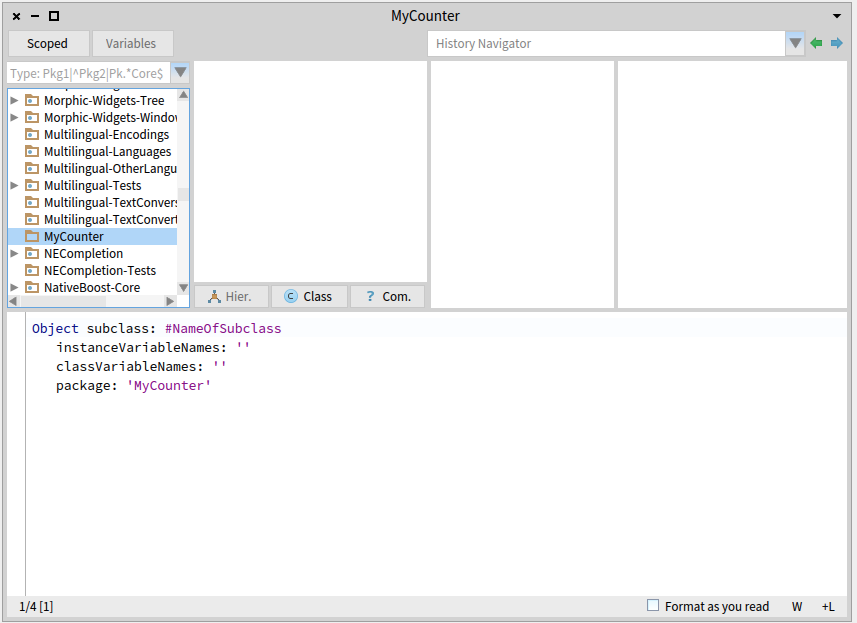
\includegraphics[width=1.0\textwidth]{/Users/ducasse/Workspace/FirstCircle/MyBooks/Bk-Writing/PharoBooks/LearningOOPWithPharoTrans/_result/pdf/Chapters/Counter/figures/CounterPackageCreated.png}\caption{Package created and class creation template.\label{figpackageCreated}}\end{center}
\end{figure}

\section{Create your own class}
In this part, you will create your first class. In Pharo, a class is defined in a package. You will create a package then a class. The steps we will do are the same ones every time you create a class, so memorize them well. 
\subsection{Create a package}
Using the Browser create a package. The system will ask you a name, write \textcode{MyCounter}. This new package is then created and added to the list. Figure \ref{figpackageCreated} shows the result of creating such a package.
\subsection{Create a class}
Creating a class requires four steps. They consist basically in editing the class definition template to specify the class you want to create.

\begin{itemize}
\item By default, the system helps you to define a subclass of the class \textcode{Object}. This is why it is written \textcode{Object subclass: \#NameOfSubclass}.
\end{itemize}

\begin{itemize}
\item \textbf{Class Name.} You should fill in the name of your class by replacing the word \textcode{NameOfSubclass} with the word \textcode{Counter}. Take care that the name of the class starts with a capital letter and that you do not remove the \#sign in front of \textcode{NameOfClass}. This is because the class we want to create does not exist yet, so we have to give its name, and we use a Symbol (a unique string in Pharo) to do so. 
\end{itemize}

\begin{itemize}
\item \textbf{Instance variable definition.} Then, you should fill in the names of the instance variables of this class. We need one instance variable called \textcode{count}. Take care that you leave the string quotes!
\end{itemize}

\begin{itemize}
\item \textbf{Class variable definition}. As we do not need any class variable make sure that the argument  for the class instance variables is an empty string \textcode{classInstanceVariableNames: ''}.
\end{itemize}

You should get the following class definition.

\begin{displaycode}{plain}
Object subclass: #Counter
   instanceVariableNames: 'count'
   classVariableNames: ''
   package: 'MyCounter'
\end{displaycode}

Now we should compile it. We now have a filled-in class definition for the class \textcode{Counter}. To define it, we still have to \textit{compile} it. Therefore, select the accept menu item. The class \textcode{Counter} is now compiled and immediately added to the system.

Figure \ref{figclassCreated} illustrates the resulting situation that the browser should show.

\begin{figure}

\begin{center}
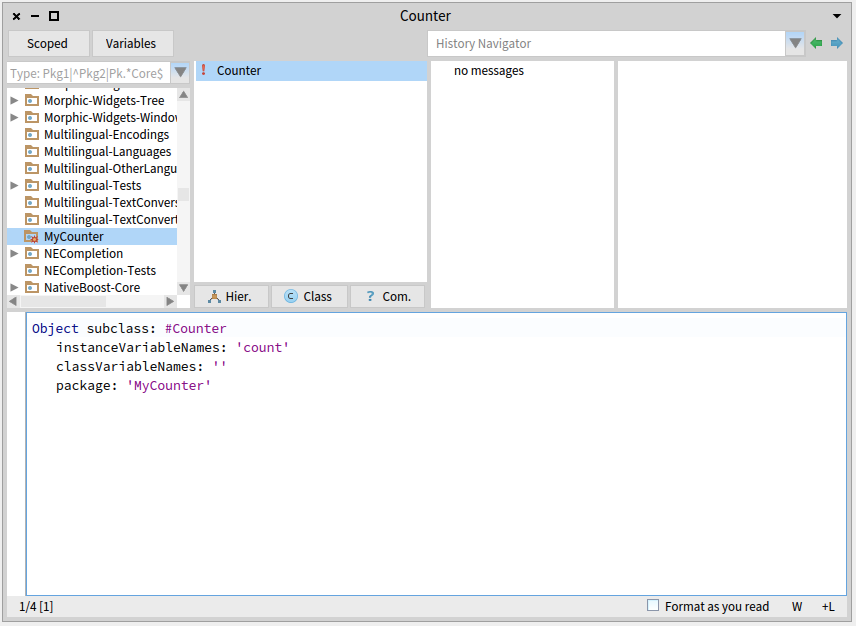
\includegraphics[width=1.0\textwidth]{/Users/ducasse/Workspace/FirstCircle/MyBooks/Bk-Writing/PharoBooks/LearningOOPWithPharoTrans/_result/pdf/Chapters/Counter/figures/CounterClassCreated.png}\caption{Class created.\label{figclassCreated}}\end{center}
\end{figure}


The tool runs automatically some code critic and some of them are just inaccurate, so do not care for now. 

As we are disciplined developers, we add a comment to \textcode{Counter} class by clicking Comment button. You can write the following comment:

\begin{displaycode}{plain}
Counter is a simple concrete class which supports incrementing and decrementing a counter.
Its API is 
- decrement, increment
- count
Its creation API is message withValue: 
\end{displaycode}

Select menu item 'accept' to store this class comment in the class.
\section{Define protocols and methods}
In this part you will use the browser to learn how to add protocols and methods.

The class we have defined has one instance variable named \textcode{count}. You should remember that in Pharo, (1) everything is an object, (2)  instance variables are private to the object, and (3) the only way to interact with an object is by sending messages to it.

Therefore, there is no other mechanism to access the instance variable values from outside an object than sending a message to the object. What you can do is to define messages that return the value of the instance variable. Such methods are called \textit{accessors}, and it is a common practice to always define and use them. We start to create an accessor method for our instance variable \textcode{count}.

A method is usually sorted into a protocol. These protocols are just a group of methods without any language semantics, but convey important navigation information for the reader of your class. You get protocol named: \textcode{'testing'} for method performing tests, \textcode{'printing'} for methods displaying the object, \textcode{'accessing'} for simple accessor methods and so on. 

Although protocols can have any name, Pharo programmers follow certain conventions for naming these protocols. But don't be stressed if you do not name well your protocols. 
\subsection{Create a method}
Now let us create the accessor methods for the instance variable \textcode{count}. Start by selecting the class \textcode{Counter} in a browser, and make sure that you are editing the instance side of the class (i.e., we define methods that will be sent to instances) by deselecting the Class side radio button.

Create a new protocol by bringing the menu of methods protocol list: click on the third list from the left. Select the newly created protocol. Then in the bottom pane, the edit field displays a method template laying out the default structure of a method. As a general hint, double click at the end of or beginning of the text and start typing your method.
Replace the template with the following method definition:

\begin{displaycode}{plain}
count
   "return the current value of the value instance variable"
   ^ count
\end{displaycode}

This defines a method called \textcode{count}, taking no arguments, having a method comment and returning the instance variable \textcode{count}. Then choose \textit{accept} in the menu to compile the method. You can now test your new method by typing and evaluating the next expression in a Playground, or any text editor.

\begin{displaycode}{plain}
Counter new count
>>> nil
\end{displaycode}

This expression first creates a new instance of \textcode{Counter}, and then sends the message \textcode{count} to it. It retrieves the current value of the counter. This should return \textcode{nil} (the default value for non-initialised instance variables). Afterwards we will create instances with a reasonable default initialisation value.
\subsection{Adding a setter method}
Another method that is normally used besides the accessor method is a so-called setter method. Such a method is used to change the value of an instance variable from a client. For example, the expression \textcode{Counter new count: 7} first creates a new \textcode{Counter} instance and then sets its value to 7:

The snippets shows that the counter effectively contains its value.

\begin{displaycode}{plain}
| c |
c := Counter new count: 7.
c count
>>> 7
\end{displaycode}

This setter method does not currently exist, so as an exercise write the method \textcode{count:} such that, when invoked on an instance of \textcode{Counter},  instance variable is set to the argument given to the message. Test your method by typing and evaluating the expression above.
\section{Define a Test Class}
Writing tests is an important activity that will support the evolution of your application. Remember that a test is written \textit{once and executed million} times. For example if we have turned the expression above into a test we could have checked automatically that our new method is correctly working. 

To define a test case we will define a class that inherits from \textcode{TestCase}. Therefore define a class named \textcode{CounterTest} as follows:

\begin{displaycode}{plain}
TestCase subclass: #CounterTest
   instanceVariableNames: ''
   classVariableNames: ''
   package: 'MyCounter'
\end{displaycode}

Now we can write a first test by defining one method. Test methods should start with \textit{test} to be automatically executed by the TestRunner or when you press on the icon of the method. Now to make sure that you understand in which class we define the method we prefix the method body with the class name and \textcode{\textgreater{}\textgreater{}}.
\textcode{CounterTest\textgreater{}\textgreater{}} means that the method is defined in the class \textcode{CounterTest}.

Define the following method. It first creates an instance, sets its value and verifies that the value is correct. The message \textcode{assert:} is a special message verifying if the test passed or not.

\begin{displaycode}{plain}
CounterTest >> testCountIsSetAndRead
   | c |
   c := Counter new.
   c count: 7.
   self assert: c count = 7
\end{displaycode}

Verify that the test passes by executing either pressing the icon in front of the method or using the TestRunner available in the Tools menu (selecting your package).
Since you have a first green test. This is a good moment to save your work. 


\begin{figure}

\begin{center}
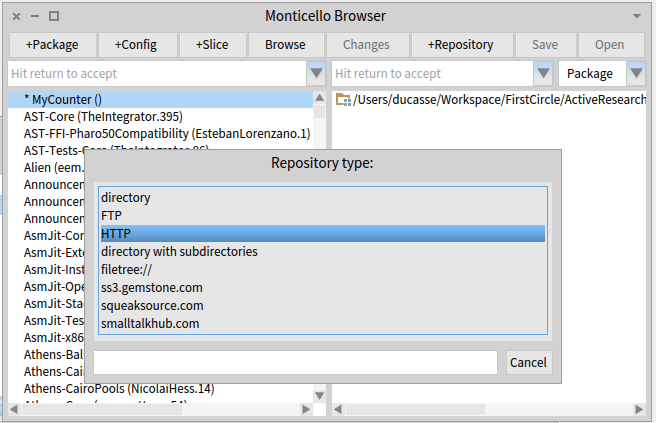
\includegraphics[width=1.0\textwidth]{/Users/ducasse/Workspace/FirstCircle/MyBooks/Bk-Writing/PharoBooks/LearningOOPWithPharoTrans/_result/pdf/Chapters/Counter/figures/CounterAddingRepo.png}\caption{Selecting a new kind of repository to the list of possible places to commit the package.\label{figSelectingARepo}}\end{center}
\end{figure}



\begin{figure}

\begin{center}
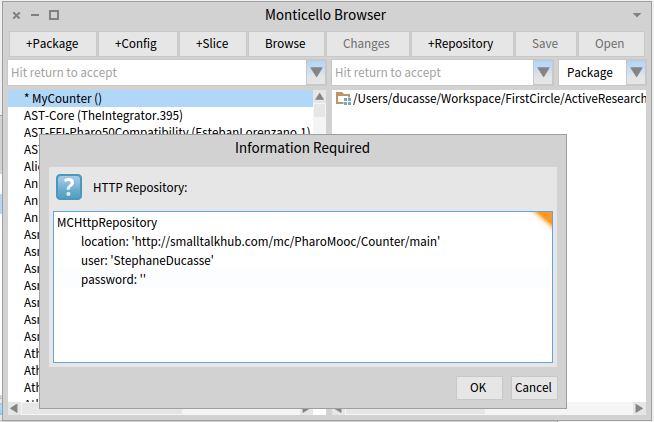
\includegraphics[width=1.0\textwidth]{/Users/ducasse/Workspace/FirstCircle/MyBooks/Bk-Writing/PharoBooks/LearningOOPWithPharoTrans/_result/pdf/Chapters/Counter/figures/CounterEditingProject.png}\caption{Editing the repository information.\label{figAddingARepo}}\end{center}
\end{figure}

\section{Saving your work}
Several ways to save your work exist. 

\begin{itemize}
\item \textit{Using plain files}. You can save the class or a method by clicking on it and selecting the fileout menu item. You will get a file containing the source code on your hard-disk - This is not the favorite way to save your code. 
\item \textit{Using a version control system}. It is better to use a version control system. In Pharo you can use Monticello and Git (even if it is more for advanced users).
\end{itemize}

In this chapter, we explain the simplest way to get you done. Note that the complete set of Pharo packages is managed via Monticello (which is a distributed versioning control system - there are chapters in \textbf{Pharo by Example} and \textbf{Deep into Pharo} books \url{http://books.pharo.org}).

Use the \textbf{Monticello Browser} (available in Tools) to save your work. You can save a package locally on your hard-disk or on a remote server on the web such as \url{http://www.smalltalkhub.com}
\subsection{Saving using Monticello}
Using Monticello you can save your work:

\begin{itemize}
\item \textit{Locally}. You can store your packages in a folder on your disk (use directory as a kind of repository below).
\item \textit{Remotely}. Using an account on a free server such \url{http://www.smalltalkhub.com/}. You can save your work and share it with others.
\end{itemize}

Note each time you load or save a package, this package is also be stored in the folder named 'package-cache' on your hard-disk.
\subsubsection{Add a repository}
Go to \url{http://www.smalltalkhub.com/} and create a member account then register a new project. You get an HTTP entry that refers to your project. Define a new HTTP repository using the Monticello Browser as shown by Figures \ref{figSelectingARepo} and \ref{figAddingARepo}.

Figure \ref{figSelectingARepo} shows that your package is dirty: this is indicated with the little '*' in front of the packages.

\textbf{Example.} As authors we  are saving the examples for this chapter as a special team named PharoMooc in the Counter project so our information is the following:  

\begin{displaycode}{plain}
MCHttpRepository
	location: 'http://smalltalkhub.com/mc/PharoMooc/Counter/main'
	user: ''
	password: ''
\end{displaycode}

Now for you, you should adapt the following template to use your own information: 

\begin{displaycode}{plain}
MCHttpRepository
	location: 'http://smalltalkhub.com/mc/YourAccount/YourProject/main'
	user: 'YourAccountID'
	password: 'YourAccountPassword'
\end{displaycode}
\subsubsection{Saving your package}
To save your work, simply select your package and the repository you want to save it to and save it using the Save button. This will open a dialog where you can give a comment, version numbers and blessing. From then on, other people can load it from there, in the same way that you would use cvs or other multi-user versioning systems. Saving the image is also a way to save your working environment, but not a way to version and publish it in a way that can be easily shared.

You can of course both publish your package (so that other people can load it, and that you can compare it with other versions, etc.) and save your image (so that next time that you start your image you are in the same working environment).
\section{Adding more messages}
Before implementing the following messages we define first a test.
We define one test for the method \textcode{increment} as follows:

\begin{displaycode}{plain}
CounterTest >> testIncrement
   | c |
   c := Counter new.
   c count: 0 ; increment; increment.
   self assert: c count = 2
\end{displaycode}

Here we create a counter, set its value to 0, send it the message increment two times and verify that we get a counter of value 2. 

Now you should implement some more methods. 

\begin{itemize}
\item Propose a definition for the method \textcode{increment} and implement it. 
\item Implement also a new test method for the method \textcode{decrement}.
\item Define the method \textcode{decrement} place it together with \textcode{increment} in the protocol \textcode{'operation'}.
\end{itemize}

Here are the possible definitions for such methods. 

\begin{displaycode}{plain}
Counter >> increment
   count := count + 1
\end{displaycode}

\begin{displaycode}{plain}
Counter >> decrement
   count := count - 1
\end{displaycode}


\begin{figure}

\begin{center}
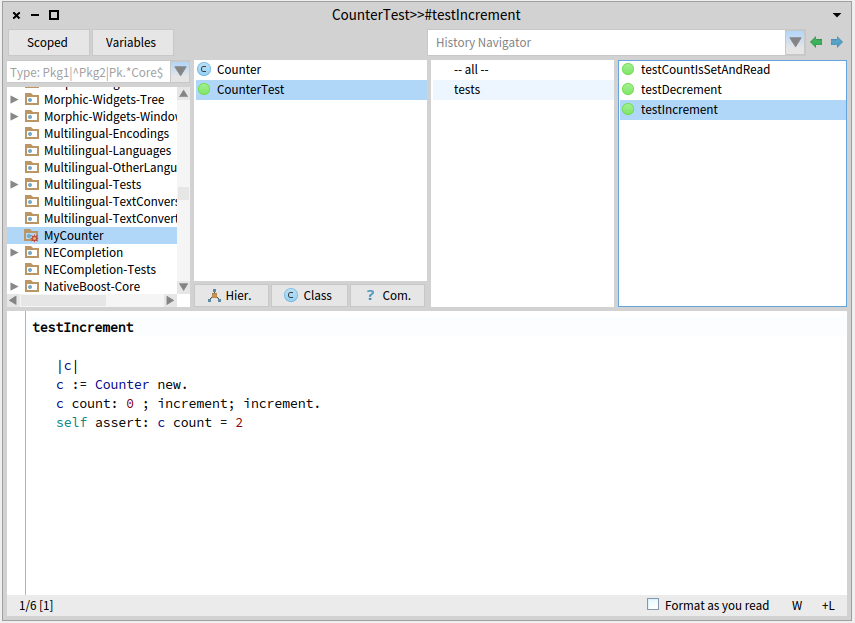
\includegraphics[width=1.0\textwidth]{/Users/ducasse/Workspace/FirstCircle/MyBooks/Bk-Writing/PharoBooks/LearningOOPWithPharoTrans/_result/pdf/Chapters/Counter/figures/CounterClassTestCreated.png}\caption{Class with green tests.\label{figclassTestCreated}}\end{center}
\end{figure}


Run your tests they should pass (as shown in Figure \ref{figclassTestCreated}). Again this is a good moment to save your work. Saving at point where tests are green
is always a good process. 
\section{Better object description}
When you select the expression \textcode{Counter new} and print its result (using the Print it menu of the editor) you obtain a simple string \textcode{'a Counter'}.

\begin{displaycode}{plain}
Counter new
>>> a Counter
\end{displaycode}

We would like to get a much richer information for example knowing the counter value. Implement the following methods in the protocol \textcode{printing}

\begin{displaycode}{plain}
Counter >> printOn: aStream
   super printOn: aStream.
   aStream nextPutAll: ' with value: ', self count printString.
\end{displaycode}

Note that the method \textcode{printOn:} is used when you print an object using print it (See Figure \ref{figBetterDescription}). In addition this method is invoked when you click on \textcode{self} in an inspector. An inspector is an object to interact and modify objects. It is really powerful during development.


\begin{figure}

\begin{center}
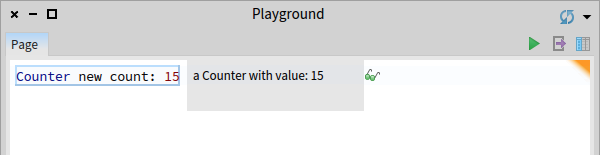
\includegraphics[width=1.0\textwidth]{/Users/ducasse/Workspace/FirstCircle/MyBooks/Bk-Writing/PharoBooks/LearningOOPWithPharoTrans/_result/pdf/Chapters/Counter/figures/CounterBetterDescription.png}\caption{Better description doing a Print It (cmd + P).\label{figBetterDescription}}\end{center}
\end{figure}

\section{Instance initialization method}
Right now the initial value of our counter is not set as the following expression shows it.

\begin{displaycode}{plain}
Counter new count
>>> nil
\end{displaycode}

Let us write a test checking that a newly created instance has 0 as a default value.

\begin{displaycode}{plain}
CounterTest >> testValueAtCreationTimeIsZero
   self assert: Counter new count = 0
\end{displaycode}

If you run it, it will turn yellow indicating a failure (a situation that you anticipated but that is not correct) - by opposition to an error which is an anticipated situation leading to failed assertion. 
\subsection{Define an initialize method}
Now we have to write an initialization method that sets a default value of the \textcode{count} instance variable. However, as we mentioned the \textcode{initialize} message is sent to the newly created instance. This means that the \textcode{initialize} method should be defined at the instance side as any method that is sent to an instance of \textcode{Counter} (like \textcode{increment}) and \textcode{decrement}. The \textcode{initialize} method is responsible to set up the default value of instance variables.

Therefore at the instance side, you should create a protocol \textcode{initialization}, and create the following method (the body of this method is left blank. Fill it in!).

\begin{displaycode}{plain}
Counter >> initialize
  "set the initial value of the value to 0"
  
  count := 0
\end{displaycode}

Now create a new instance of class \textcode{Counter}. Is it initialized by default? The following code should now work without problem:

\begin{displaycode}{plain}
Counter new increment
\end{displaycode}

and the following one should return 2

\begin{displaycode}{plain}
Counter new increment; increment; count
>>> 2
\end{displaycode}

Again save your work
\section{Conclusion}
In this chapter you learned how to define packages, classes, methods, and define tests.
The flow of programming that we chose for this first tutorial is similar to most of programming languages.
In Pharo you can use a different flow that is based on defining a test first, executing it and when the execution raises error to define the corresponding classes, methods, and instance variables often from inside the debugger. We suggest you now to redo the exercise following the second companion video.



% lulu requires an empty page at the end. That's why I'm using
% \backmatter here.
\backmatter

% Index would go here
\bibliographystyle{abbrv}
\bibliography{others.bib}
\end{document}
